\documentclass[]{ctexbook}
\usepackage{lmodern}
\usepackage{amssymb,amsmath}
\usepackage{ifxetex,ifluatex}
\usepackage{fixltx2e} % provides \textsubscript
\ifnum 0\ifxetex 1\fi\ifluatex 1\fi=0 % if pdftex
  \usepackage[T1]{fontenc}
  \usepackage[utf8]{inputenc}
\else % if luatex or xelatex
  \ifxetex
    \usepackage{xltxtra,xunicode}
  \else
    \usepackage{fontspec}
  \fi
  \defaultfontfeatures{Ligatures=TeX,Scale=MatchLowercase}
\fi
% use upquote if available, for straight quotes in verbatim environments
\IfFileExists{upquote.sty}{\usepackage{upquote}}{}
% use microtype if available
\IfFileExists{microtype.sty}{%
\usepackage{microtype}
\UseMicrotypeSet[protrusion]{basicmath} % disable protrusion for tt fonts
}{}
\usepackage[b5paper,paperwidth=17cm,paperheight=24cm,tmargin=3cm,bmargin=2.4cm,lmargin=3cm,rmargin=2cm]{geometry}
\usepackage[unicode=true]{hyperref}
\hypersetup{
            pdftitle={Steem Engine Handbook},
            pdfauthor={Steem 中文社区集体创作},
            pdfborder={0 0 0},
            breaklinks=true}
\urlstyle{same}  % don't use monospace font for urls
\usepackage{natbib}
\bibliographystyle{apalike}
\usepackage{longtable,booktabs}
% Fix footnotes in tables (requires footnote package)
\IfFileExists{footnote.sty}{\usepackage{footnote}\makesavenoteenv{long table}}{}
\usepackage{graphicx,grffile}
\makeatletter
\def\maxwidth{\ifdim\Gin@nat@width>\linewidth\linewidth\else\Gin@nat@width\fi}
\def\maxheight{\ifdim\Gin@nat@height>\textheight\textheight\else\Gin@nat@height\fi}
\makeatother
% Scale images if necessary, so that they will not overflow the page
% margins by default, and it is still possible to overwrite the defaults
% using explicit options in \includegraphics[width, height, ...]{}
\setkeys{Gin}{width=\maxwidth,height=\maxheight,keepaspectratio}
\IfFileExists{parskip.sty}{%
\usepackage{parskip}
}{% else
\setlength{\parindent}{0pt}
\setlength{\parskip}{6pt plus 2pt minus 1pt}
}
\setlength{\emergencystretch}{3em}  % prevent overfull lines
\providecommand{\tightlist}{%
  \setlength{\itemsep}{0pt}\setlength{\parskip}{0pt}}
\setcounter{secnumdepth}{5}
% Redefines (sub)paragraphs to behave more like sections
\ifx\paragraph\undefined\else
\let\oldparagraph\paragraph
\renewcommand{\paragraph}[1]{\oldparagraph{#1}\mbox{}}
\fi
\ifx\subparagraph\undefined\else
\let\oldsubparagraph\subparagraph
\renewcommand{\subparagraph}[1]{\oldsubparagraph{#1}\mbox{}}
\fi

% set default figure placement to htbp
\makeatletter
\def\fps@figure{htbp}
\makeatother

\usepackage{pdfpages}
\usepackage{wasysym} % insert a smiling and frowning face

\usepackage{booktabs}
\usepackage{longtable}

\usepackage{indentfirst}
\setlength{\parindent}{2em}

\usepackage{framed,color}
\definecolor{shadecolor}{RGB}{248,248,248}

\renewcommand{\textfraction}{0.05}
\renewcommand{\topfraction}{0.8}
\renewcommand{\bottomfraction}{0.8}
\renewcommand{\floatpagefraction}{0.75}

\let\oldhref\href
\renewcommand{\href}[2]{#2\footnote{\url{#1}}}


% \makeatletter
% \newenvironment{kframe}{%
% \medskip{}
% \setlength{\fboxsep}{.8em}
 % \def\at@end@of@kframe{}%
 % \ifinner\ifhmode%
  % \def\at@end@of@kframe{\end{minipage}}%
  % \begin{minipage}{\columnwidth}%
 % \fi\fi%
 % \def\FrameCommand##1{\hskip\@totalleftmargin \hskip-\fboxsep
 % \colorbox{shadecolor}{##1}\hskip-\fboxsep
     % % There is no \\@totalrightmargin, so:
     % \hskip-\linewidth \hskip-\@totalleftmargin \hskip\columnwidth}%
 % \MakeFramed {\advance\hsize-\width
   % \@totalleftmargin\z@ \linewidth\hsize
   % \@setminipage}}%
 % {\par\unskip\endMakeFramed%
 % \at@end@of@kframe}
% \makeatother

% \renewenvironment{Shaded}{\begin{kframe}}{\end{kframe}}

\usepackage{makeidx}
\makeindex

\urlstyle{tt}

\usepackage{amsthm}
\makeatletter
\def\thm@space@setup{%
 \thm@preskip=8pt plus 2pt minus 4pt
 \thm@postskip=\thm@preskip
}
\makeatother


%%%%%%%%%% 生成小贴士目录
% \usepackage{etoolbox}
% \usepackage{amsthm}
% \newtheoremstyle{mystyle}
% {\topsep}{\topsep}{}{}{\bfseries}{:}{\newline}
% {\thmname{#1}\thmnumber{ #2}\thmnote{ (#3)}%
	% \ifstrempty{#3}%
	% {\addcontentsline{def}{subsection}{#1~\themydef}}%
	% {\addcontentsline{def}{subsection}{#1~\themydef~(#3)}}}
% \theoremstyle{mystyle}
% \newtheorem{mydef}{小贴士}
% \makeatletter
% \newcommand\definitionname{小贴士}
% \newcommand\listdefinitionname{小贴士目录}
% \newcommand\listofdefinitions{%
	% \section*{\listdefinitionname}\@starttoc{mydef}}
% \makeatother

\ifxetex
  \usepackage{letltxmacro}
  \setlength{\XeTeXLinkMargin}{1pt}
  \LetLtxMacro\SavedIncludeGraphics\includegraphics
  \def\includegraphics#1#{% #1 catches optional stuff (star/opt. arg.)
    \IncludeGraphicsAux{#1}%
  }%
  \newcommand*{\IncludeGraphicsAux}[2]{%
    \XeTeXLinkBox{%
      \SavedIncludeGraphics#1{#2}%
    }%
  }%
\fi

\newenvironment{rmdblock}[1]
  {\begin{shaded*}
  \begin{itemize}
  \renewcommand{\labelitemi}{
    \raisebox{-.7\height}[0pt][0pt]{
      {\setkeys{Gin}{width=2em,keepaspectratio}\includegraphics{images/icons/#1}}
    }
  }
  \item
  }
  {
  \end{itemize}
  \end{shaded*}
  }
\newenvironment{rmdcaution}
  {\begin{rmdblock}{caution}}
  {\end{rmdblock}}
\newenvironment{rmdinsight}
  {\begin{rmdblock}{insight}}
  {\end{rmdblock}}
\newenvironment{rmdexercise}
  {\begin{rmdblock}{exercise}}
  {\end{rmdblock}}
\newenvironment{rmdexample}
  {\begin{rmdblock}{exeample}}
  {\end{rmdblock}}
\newenvironment{rmdtip}
  {\begin{rmdblock}{tip}}
  {\end{rmdblock}}


%%%%%%% 引用 verbatim 的换行问题
\usepackage{etoolbox}
\usepackage{verbatim}
\makeatletter
\def\@xobeysp{\ }% Or just a space, with a different result
\let\verbatim@nolig@list\empty
\appto\verbatim@font{\raggedright}
\makeatother


\usepackage{xeCJK}% You'd better use the latest version%
%\setCJKmainfont{NSimSun}
\xeCJKsetup{Verb=false}
\normalspacedchars{}
\ExplSyntaxOn
% Hack into xeCJK package if you want to allow linebreaks after (almost) any character.
% Delete this if you don't want that.
\tex_chardef:D \c_fifty = 50 ~
\xeCJK_inter_class_toks:nnn { Default } { Default } { \tex_penalty:D \c_one_hundred }
\xeCJK_inter_class_toks:nnn { Default } { HalfLeft } { \tex_penalty:D \c_fifty }
\xeCJK_inter_class_toks:nnn { Default } { HalfRight } { \tex_penalty:D \c_one_thousand }
\xeCJK_inter_class_toks:nnn { HalfLeft } { Default } { \tex_penalty:D \c_one_thousand }
\xeCJK_inter_class_toks:nnn { HalfLeft } { HalfLeft } { \tex_penalty:D \c_one_thousand }
\xeCJK_inter_class_toks:nnn { HalfLeft } { HalfRight } { \tex_penalty:D \c_one_thousand }
\xeCJK_inter_class_toks:nnn { HalfRight } { Default } { \tex_penalty:D \c_fifty }
\xeCJK_inter_class_toks:nnn { HalfRight } { HalfLeft } { \tex_penalty:D \c_fifty }
\xeCJK_inter_class_toks:nnn { HalfRight } { HalfRight } { \tex_penalty:D \c_one_thousand }
\ExplSyntaxOff
%%%%%%%%%%%%%%%%%%%%%%%%%%%%%%%%%%%%%%%%%%%%%%%%%%%%%%%%%%%%%%%%
% \usepackage{gchords}

% \newcommand\mychords{
% \def\chordsize{1.6mm}   % distance between two frets (and two strings)
% \font\fingerfont=cmr5  % font used for numbering fingers
% \font\namefont=cmr10    % font used for labeling of the chord
% \font\fretposfont=cmr7  % font used for the fret position marker
% \def\dampsymbol{{\tiny$\scriptstyle\times$}} %  `damp this string' marker
% }

% \renewcommand\yoff{3}
% \renewcommand\fingsiz{1.6}

% % upchord
% \newcommand{\AsevenMaj}{\upchord{\chord{t}{x,n,p2,p1,p2,n}{A7+}}}
% \newcommand{\Aseven}{\upchord{\chord{t}{x,n,p2,n,p2,n}{A7}}}
% \newcommand{\A}{\upchord{\chord{t}{x,n,p2,p2,p2,n}{A}}}
% \newcommand{\Am}{\upchord{\chord{t}{n,n,p2,p2,p1,n}{Am}}}
% \newcommand{\Amfive}{\upchord{\chord{{5~}}{p1,p3,p3,p1,p1,p1}{Am(5)}}}
% \newcommand{\Bb}{\upchord{\chord{t}{f1p1,f1p1,p3,p3,p3,f1p1}{$^b$B}}}
% \newcommand{\BmseveN}{\upchord{\chord{t}{x,p2,p4,p3,p3,p2}{Bm7+}}}
% \newcommand{\BmsevenA}{\upchord{\chord{t}{x,n,p4,p4,p3,n}{Bm/A}}}
% \newcommand{\Bmseven}{\upchord{\chord{t}{x,p2,p4,p2,p3,p2}{Bm7}}}
% \newcommand{\Bm}{\upchord{\chord{t}{x,p2,p4,p4,p3,p2}{Bm}}}
% \newcommand{\BM}{\upchord{\chord{t}{f1p2,f1p2,p4,p4,p4,f1p2}{B}}}
% \newcommand{\Bseven}{\upchord{\chord{t}{x,f1p2,p4,f1p2,p4,f1p2,}{B7}}}
% \newcommand{\BMseven}{\upchord{\chord{t}{n,p2,p1,p2,n,p2}{B7}}}
% \newcommand{\BsevenBasDs}{\upchord{\chord{t}{x,x,p1,p2,n,p2}{B7/D\#}}}
% \newcommand{\CM}{\upchord{\chord{t}{n,p3,p2,n,p1,n}{C}}}
% \newcommand{\CssevenLight}{\upchord{\chord{t}{x,p4,p3,p4,p2,x}{C\#7}}}
% \newcommand{\Csthree}{\upchord{\chord{{4~}}{f1p1,f1p1,p3,p3,p3,f1p1}{$^\#$C}}}
% \newcommand{\Cthree}{\upchord{\chord{{3~}}{f1p1,f1p1,p3,p3,p3,f1p1}{C(3)}}}
% \newcommand{\Cseven}{\upchord{\chord{t}{n,p3,p2,p3,p1,n}{C7}}}
% \newcommand{\Cm}{\upchord{\chord{t}{f1p3,f1p3,p5,p5,p4,f1p3}{Cm}}}
% \newcommand{\Csm}{\upchord{\chord{{4~}}{f1p1,f1p1,p3,p3,p2,f1p1}{\#Cm}}}
% \newcommand{\DmBasB}{\upchord{\chord{t}{x,p2,p3,p2,p3,x}{Dm/B}}}
% \newcommand{\DseveN}{\upchord{\chord{t}{x,x,n,p2,p2,p2}{D7+}}}
% \newcommand{\Dseven}{\upchord{\chord{t}{x,x,n,p2,p1,p2}{D7}}}
% \newcommand{\Dsix}{\upchord{\chord{t}{x,x,n,p2,n,p2}{D6}}}
% \newcommand{\D}{\upchord{\chord{t}{x,x,n,p2,p3,p2}{D}}}
% \newcommand{\Dm}{\upchord{\chord{t}{x,x,n,p2,p3,p1}{Dm}}}
% \newcommand{\Eb}{\upchord{\chord{{6~}}{f1p1,f1p1,p3,p3,p3,f1p1}{$^b$E}}}
% \newcommand{\E}{\upchord{\chord{t}{n,p2,p2,p1,n,n}{E}}}
% \newcommand{\Eseven}{\upchord{\chord{{7~}}{f1p1,f1p1,p3,p3,p3,f1p1}{E(7)}}}
% \newcommand{\EseveNNine}{\upchord{\chord{t}{n,f1p2,f1p2,p4,p3,f1p2,}{E79}}}
% \newcommand{\EseveN}{\upchord{\chord{t}{n,p2,p2,p4,p3,p4}{E7}}}
% \newcommand{\EsevenFour}{\upchord{\chord{t}{n,p2,p2,p4,p3,p5}{E7,11}}}
% \newcommand{\Em}{\upchord{\chord{t}{n,p2,p2,n,n,n}{Em}}}
% \newcommand{\F}{\upchord{\chord{t}{f1p1,p3,p3,p2,f1p1,f1p1}{F}}}
% \newcommand{\Fs}{\upchord{\chord{t}{f2p2,p4,p4,p3,f1p2,f1p2}{F\#}}}
% \newcommand{\Fsmin}{\upchord{\chord{t}{f1p2,p4,p4,f1p2,f1p2,f1p2,}{F\#m}}}
% \newcommand{\FsminLight}{\upchord{\chord{t}{x,x,f3p4,f1p2,f1p2,f1p2,}{F\#m}}}
% \newcommand{\FsminBasSeveN}{\upchord{\chord{t}{x,x,f3p3,f1p2,f1p2,f1p2,}{F\#m/E\#}}}
% \newcommand{\FsminBasSeven}{\upchord{\chord{t}{x,x,f2p2,f1p2,f1p2,f1p2,}{F\#m/E}}}
% \newcommand{\FsminSeven}{\upchord{\chord{t}{f1p2,p4,p4,f1p2,p5,f1p2,}{F\#7m}}}
% \newcommand{\GM}{\upchord{\chord{t}{p3,p2,n,n,n,p3}{G}}}
% \newcommand{\Gsminseven}{\upchord{\chord{t}{f2p4,x,f4p4,f4p4,f4p4,f4p4,}{G\#7}}}
% \newcommand{\Gthree}{\upchord{\chord{t}{f1p3,p5,p5,p4,f1p3,f1p3}{G(3)}}}
% \newcommand{\Gm}{\upchord{\chord{{3~}}{f1p1,p3,p3,f1p1,f1p1,f1p1}{Gm}}}
% \newcommand{\Gsm}{\upchord{\chord{{4~}}{f1p1,p3,p3,f1p1,f1p1,f1p1}{\#Gm}}}
% \newcommand{\Gseven}{\upchord{\chord{t}{p3,p2,n,n,n,p1}{G7}}}

% %inline 
% \newcommand{\iAsevenMaj}{\chord{t}{x,n,p2,p1,p2,n}{A7+}}
% \newcommand{\iAseven}{\chord{t}{x,n,p2,n,p2,n}{A7}}
% \newcommand{\iA}{\chord{t}{x,n,p2,p2,p2,n}{A}}
% \newcommand{\iAm}{\chord{t}{n,n,p2,p2,p1,n}{Am}}
% \newcommand{\iAmfive}{\chord{{5~}}{p1,p3,p3,p1,p1,p1}{Am(5)}}
% \newcommand{\iBb}{\chord{t}{f1p1,f1p1,p3,p3,p3,f1p1}{$^b$B}}
% \newcommand{\iBmseveN}{\chord{t}{x,p2,p4,p3,p3,p2}{Bm7+}}
% \newcommand{\iBmsevenA}{\chord{t}{x,n,p4,p4,p3,n}{Bm/A}}
% \newcommand{\iBmseven}{\chord{t}{x,p2,p4,p2,p3,p2}{Bm7}}
% \newcommand{\iBm}{\chord{t}{x,p2,p4,p4,p3,p2}{Bm}}
% \newcommand{\iBM}{\chord{t}{f1p2,f1p2,p4,p4,p4,f1p2}{B}}
% \newcommand{\iBseven}{\chord{t}{x,f1p2,p4,f1p2,p4,f1p2,}{B7}}
% \newcommand{\iBMseven}{\chord{t}{n,p2,p1,p2,n,p2}{B7}}
% \newcommand{\iBsevenBasDs}{\chord{t}{x,x,p1,p2,n,p2}{B7/D\#}}
% \newcommand{\iCM}{\chord{t}{n,p3,p2,n,p1,n}{C}}
% \newcommand{\iCssevenLight}{\chord{t}{x,p4,p3,p4,p2,x}{C\#7}}
% \newcommand{\iCsthree}{\chord{{4~}}{f1p1,f1p1,p3,p3,p3,f1p1}{$^\#$C}}
% \newcommand{\iCthree}{\chord{{3~}}{f1p1,f1p1,p3,p3,p3,f1p1}{C(3)}}
% \newcommand{\iCseven}{\chord{t}{n,p3,p2,p3,p1,n}{C7}}
% \newcommand{\iCm}{\chord{t}{f1p3,f1p3,p5,p5,p4,f1p3}{Cm}}
% \newcommand{\iCsm}{\chord{{4~}}{f1p1,f1p1,p3,p3,p2,f1p1}{\#Cm}}
% \newcommand{\iDmBasB}{\chord{t}{x,p2,p3,p2,p3,x}{Dm/B}}
% \newcommand{\iDseveN}{\chord{t}{x,x,n,p2,p2,p2}{D7+}}
% \newcommand{\iDseven}{\chord{t}{x,x,n,p2,p1,p2}{D7}}
% \newcommand{\iDsix}{\chord{t}{x,x,n,p2,n,p2}{D6}}
% \newcommand{\iD}{\chord{t}{x,x,n,p2,p3,p2}{D}}
% \newcommand{\iDm}{\chord{t}{x,x,n,p2,p3,p1}{Dm}}
% \newcommand{\iEb}{\chord{{6~}}{f1p1,f1p1,p3,p3,p3,f1p1}{$^b$E}}
% \newcommand{\iE}{\chord{t}{n,p2,p2,p1,n,n}{E}}
% \newcommand{\iEseven}{\chord{{7~}}{f1p1,f1p1,p3,p3,p3,f1p1}{E(7)}}
% \newcommand{\iEseveNNine}{\chord{t}{n,f1p2,f1p2,p4,p3,f1p2,}{E79}}
% \newcommand{\iEseveN}{\chord{t}{n,p2,p2,p4,p3,p4}{E7}}
% \newcommand{\iEsevenFour}{\chord{t}{n,p2,p2,p4,p3,p5}{E7,11}}
% \newcommand{\iEm}{\chord{t}{n,p2,p2,n,n,n}{Em}}
% \newcommand{\iF}{\chord{t}{f1p1,p3,p3,p2,f1p1,f1p1}{F}}
% \newcommand{\iFs}{\chord{t}{f2p2,p4,p4,p3,f1p2,f1p2}{F\#}}
% \newcommand{\iFsmin}{\chord{t}{f1p2,p4,p4,f1p2,f1p2,f1p2,}{F\#m}}
% \newcommand{\iFsminLight}{\chord{t}{x,x,f3p4,f1p2,f1p2,f1p2,}{F\#m}}
% \newcommand{\iFsminBasSeveN}{\chord{t}{x,x,f3p3,f1p2,f1p2,f1p2,}{F\#m/E\#}}
% \newcommand{\iFsminBasSeven}{\chord{t}{x,x,f2p2,f1p2,f1p2,f1p2,}{F\#m/E}}
% \newcommand{\iFsminSeven}{\chord{t}{f1p2,p4,p4,f1p2,p5,f1p2,}{F\#7m}}
% \newcommand{\iGM}{\chord{t}{p3,p2,n,n,n,p3}{G}}
% \newcommand{\iGsminseven}{\chord{t}{f2p4,x,f4p4,f4p4,f4p4,f4p4,}{G\#7}}
% \newcommand{\iGthree}{\chord{t}{f1p3,p5,p5,p4,f1p3,f1p3}{G(3)}}
% \newcommand{\iGm}{\chord{{3~}}{f1p1,p3,p3,f1p1,f1p1,f1p1}{Gm}}
% \newcommand{\iGsm}{\chord{{4~}}{f1p1,p3,p3,f1p1,f1p1,f1p1}{\#Gm}}
%\usepackage{CJK,CJKnumb,CJKulem}  
%\newcommand{\kai}{\CJKfamily{kai}}       % 楷体
\usepackage{fancyhdr}
% Clear the header and footer
\fancyhead{}
\fancyfoot{}
\fancypagestyle{plain}{% 每章首页无页码
	\fancyhf{}
	\renewcommand{\headrulewidth}{0pt}
	\renewcommand{\footrulewidth}{0pt}
}
%\fancyhead[LE]{\small \kaishu \leftmark}
\fancyhead[LE]{\small \kaishu Steem 指南}
\fancyhead[RO]{\small \kaishu \leftmark}
\fancyfoot[LE, RO]{\thepage}
%\fancyfoot[RE]{\small \kaishu 学 R}
%\fancyfoot[LO]{\small \kaishu 零基础学习 R 语言}
%\renewcommand{\footrulewidth}{0.4pt} % 页脚横线
\pagestyle{fancy}

\frontmatter

\title{Steem Engine Handbook}
\author{Steem 中文社区集体创作}
\date{2019-06-17}

\begin{document}
%\maketitle

\begin{titlepage}
%    
\includegraphics[width=17cm]{images/cover.jpg}

\includepdf{images/cover.jpg}
\end{titlepage}

\setlength{\abovedisplayskip}{-5pt}
\setlength{\abovedisplayshortskip}{-5pt}

{
\setcounter{tocdepth}{1}
\tableofcontents
}

% \tableofcontents
% \clearpage
% \listofdefinitions

\hypertarget{index}{%
\chapter*{前言}\label{index}}
\addcontentsline{toc}{chapter}{前言}

自盘古开天地以来\ldots{}\ldots{}

\begin{quote}
(未完待续)
\end{quote}

\mainmatter

\hypertarget{start}{%
\chapter{入门 Getting Started}\label{start}}

\hypertarget{-steem-engine}{%
\section{什么是 Steem Engine?}\label{-steem-engine}}

首先,你或许可以参考 \href{https://steem-engine.com/?p=faq}{Steem Engine的FAQ} 了解它对自己的介绍 \ldots{}..

\begin{quote}
(未完待续)
\end{quote}

\hypertarget{theory}{%
\chapter{原理 Theory}\label{theory}}

\begin{enumerate}
\def\labelenumi{\arabic{enumi}.}
\tightlist
\item
  什么是 Steem Smart Contracts?
\item
  什么是 SCOT (Smart Contract Organizational Token)?
\item
  什么是 Nitrous?
\end{enumerate}

\begin{quote}
(未完待续)
\end{quote}

\hypertarget{dapp}{%
\chapter{应用 dApp}\label{dapp}}

\begin{itemize}
\tightlist
\item
  SCT
\item
  AAA
\item
  RORS
\end{itemize}

\begin{quote}
(未完待续)
\end{quote}

\hypertarget{token}{%
\chapter{货币 Token}\label{token}}

\begin{enumerate}
\def\labelenumi{\arabic{enumi}.}
\tightlist
\item
  Steem Engine 上的 Token 从何而来?
\item
  什么是 ENG?它是如何被使用的?
\item
  什么是JJM(Jiangjiangman)?它为什么火了?
\item
  什么是红包币?EMFOUR4 / EM
\item
  NBC 新手币 牛掰在哪里?
\item
  SHOP币 有几种玩法?
\end{enumerate}

\begin{quote}
(未完待续)
\end{quote}

\hypertarget{tool}{%
\chapter{工具 Tool}\label{tool}}

\begin{longtable}[]{@{}lll@{}}
\toprule
\begin{minipage}[b]{0.30\columnwidth}\raggedright
名称\strut
\end{minipage} & \begin{minipage}[b]{0.30\columnwidth}\raggedright
链接\strut
\end{minipage} & \begin{minipage}[b]{0.30\columnwidth}\raggedright
说明\strut
\end{minipage}\tabularnewline
\midrule
\endhead
\begin{minipage}[t]{0.30\columnwidth}\raggedright
Steem Engine CN版\strut
\end{minipage} & \begin{minipage}[t]{0.30\columnwidth}\raggedright
\url{https://steem-engine.netlify.com}\strut
\end{minipage} & \begin{minipage}[t]{0.30\columnwidth}\raggedright
CN区专用\strut
\end{minipage}\tabularnewline
\begin{minipage}[t]{0.30\columnwidth}\raggedright
Block Explorer\strut
\end{minipage} & \begin{minipage}[t]{0.30\columnwidth}\raggedright
\url{https://steem-engine.rocks}\strut
\end{minipage} & \begin{minipage}[t]{0.30\columnwidth}\raggedright
steem-engine的steemd\strut
\end{minipage}\tabularnewline
\begin{minipage}[t]{0.30\columnwidth}\raggedright
Token的动态\strut
\end{minipage} & \begin{minipage}[t]{0.30\columnwidth}\raggedright
\url{https://steem-engine.rocks/transactions?symbol=\%7Btoken\%7D}\strut
\end{minipage} & \begin{minipage}[t]{0.30\columnwidth}\raggedright
举例:\url{https://steem-engine.rocks/transactions?symbol=SCT}\strut
\end{minipage}\tabularnewline
\begin{minipage}[t]{0.30\columnwidth}\raggedright
账户的动态\strut
\end{minipage} & \begin{minipage}[t]{0.30\columnwidth}\raggedright
\url{https://steem-engine.rocks/@\%7Bid\%7D}\strut
\end{minipage} & \begin{minipage}[t]{0.30\columnwidth}\raggedright
举例:\href{https://steem-engine.rocks/@aggroed}{https://steem-engine.rocks/\citet{aggroed}}\strut
\end{minipage}\tabularnewline
\begin{minipage}[t]{0.30\columnwidth}\raggedright
Token的持有和锁仓\strut
\end{minipage} & \begin{minipage}[t]{0.30\columnwidth}\raggedright
\url{https://steem-engine.rocks/tokens/\%7Btoken\%7D/richlist}\strut
\end{minipage} & \begin{minipage}[t]{0.30\columnwidth}\raggedright
举例:\url{https://steem-engine.rocks/tokens/SCT/richlist}\strut
\end{minipage}\tabularnewline
\begin{minipage}[t]{0.30\columnwidth}\raggedright
交易订单\strut
\end{minipage} & \begin{minipage}[t]{0.30\columnwidth}\raggedright
\url{https://steem-engine.rocks/open_orders/@\%7Bid\%7D}\strut
\end{minipage} & \begin{minipage}[t]{0.30\columnwidth}\raggedright
举例:\href{https://steem-engine.rocks/open_orders/@aggroed}{https://steem-engine.rocks/open\_orders/\citet{aggroed}}\strut
\end{minipage}\tabularnewline
\begin{minipage}[t]{0.30\columnwidth}\raggedright
Wallet\strut
\end{minipage} & \begin{minipage}[t]{0.30\columnwidth}\raggedright
\url{https://steem-engine.com/?p=balances}\strut
\end{minipage} & \begin{minipage}[t]{0.30\columnwidth}\raggedright
举例:\url{https://steem-engine.com/?p=balances\&a=robertyan}\strut
\end{minipage}\tabularnewline
\begin{minipage}[t]{0.30\columnwidth}\raggedright
Market\strut
\end{minipage} & \begin{minipage}[t]{0.30\columnwidth}\raggedright
\url{https://steem-engine.com/?p=market\&t=\%7Btoken\%7D}\strut
\end{minipage} & \begin{minipage}[t]{0.30\columnwidth}\raggedright
举例: \url{https://steem-engine.com/?p=market\&t=SCT}\strut
\end{minipage}\tabularnewline
\begin{minipage}[t]{0.30\columnwidth}\raggedright
VP\strut
\end{minipage} & \begin{minipage}[t]{0.30\columnwidth}\raggedright
\url{https://economicstudio.github.io/vp/a=\%7Busername\%7D\&t=\%7Btoken\%7D}\strut
\end{minipage} & \begin{minipage}[t]{0.30\columnwidth}\raggedright
举例: \url{https://economicstudio.github.io/vp/?a=robertyan\&t=SCT}\strut
\end{minipage}\tabularnewline
\bottomrule
\end{longtable}

\begin{quote}
(未完待续)
\end{quote}

\hypertarget{developer}{%
\chapter{开发 Developers}\label{developer}}

\begin{itemize}
\tightlist
\item
  Steem Smart Contract: \url{https://github.com/harpagon210/steemsmartcontracts}
\item
  JavaScript Library: \url{https://github.com/harpagon210/sscjs}
\end{itemize}

\begin{quote}
(未完待续)
\end{quote}

\hypertarget{talk}{%
\chapter{杂谈 Talk}\label{talk}}

\hypertarget{steem-nature}{%
\section[区块链社交平台的本质 ]{\texorpdfstring{区块链社交平台的本质 \footnote{作者: @deanliu; 原文链接: \url{https://busy.org/@deanliu/5dxrz5}}}{区块链社交平台的本质 }}\label{steem-nature}}

原標題:【區塊鏈社交平台最重要的認識是 \ldots{}】

Steem自己是歷史上第一個\textbf{區塊鏈社交平台},存活至今3年多,在中本聰紀元裡,已經是非常長壽了\ldots{}

甚至,發展至今,社區內在自發發展下,長出了Steem Engine,推動了Steem作為\textbf{區塊鏈社交平台之基底鏈}的新紀元與可能性。(官方的SMT很可能也是這樣方向,只是可惜樓梯不太響了,人也還沒下來)

我認為這個時刻,有必要再重新想一下,到底所謂\textbf{區塊鏈社交平台},最關鍵的基礎性認識是什麼?

\begin{figure}
\centering

\includegraphics{images/chapter_07_0/woman-3373913_640.jpg}
\caption{woman-3373913\_640.jpg}
\end{figure}

什麼叫做``最關鍵的基礎性認識''呢?

就是類似一句話說出來,你就秒懂這個詞或是這件事情的本質,清晰無比。如果有個東西,讓你說上10分鐘,你都還不能說清楚這東西到底重點是什麼,那麼,有很大的概率,要嘛你不瞭解這東西,要嘛這東西並沒有什麼太大重要性。

Steem過去常常有這樣的問題,用戶們無法很清楚地告訴他們的朋友,Steem是什麼?能幹嘛?多半是囁嚅著區塊鏈社交平台這類,連他自己也說不清楚的大詞組合,鬼打牆似的重複著\ldots{} 比較好一點是說,Steem能讓你寫東西賺錢!這個好一點,可惜有騙人嫌疑,九成的人來了都賺不了夠明顯超越其時間成本的錢,那麼多離開的人就是明證。

那麼到底是什麼呢?

我認為\ldots{}. 關於\textbf{區塊鏈社交平台},最重要的認識就是 \ldots{}

\textbf{這裡不是``一般性的社交''平台,這裡是``商業性社交''平台。}

哇!我是寫到這裡才知道我會這樣寫,我自己都很驚嘆,這見解之精闢啊~~~ 哇哈哈哈~~~

是的,很多人都搞錯了。以為這裡是一般性社交平台,殊不知,這件事早已經被以facebook為首的眾多公司給做完了,做到極度競爭了\ldots{} Steem去湊著熱鬧幹嘛?取代facebook,真是化石級的笑話了\ldots{}

我認為這個認識,連創辦人Dan (BM)都沒有很精準地抓住。BM早期文章,其實是想創造一個全自由的言論環境,解放全人類的思想自由等等,你去看他早期文章很多在談這些,甚至現在EOS的Voice,可能都還有這種味道在。我現在認為,他當初這樣的想法雖然立意崇高,但是是大有問題的。

說點敏感的,6月初到最近,其實正值一些政治敏感議題之際,中文區卻蠻少人談(有一些我看到了,但不算多),要不就是用英文發。可能有些激進的人就說了,這是自我審查!但我不這麼認為,至少這不是主要因素。可是,這裡的特色不就是``抗審查''嗎?不怕打壓嗎?是的,這裡是。那麼,人們為何害怕發表自己的意見?其實,害怕或許有一些,但最主要是沒必要\ldots{}

從我上面說的就可以很簡單回答這問題:\textbf{這裡是``商業性社交''平台。}

你在職場上談政治嗎?你跟菜市場裡的販子談言論自由嗎?你跟客戶交流時,是會談你意識到的客戶的政治傾向,還是夸談自己的看法?

這不就結了?``商業''兩字,說明了一切行為。

\begin{figure}
\centering
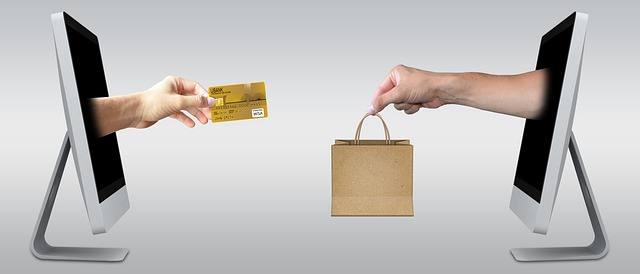
\includegraphics{images/chapter_07_0/ecommerce-2140603_640.jpg}
\caption{ecommerce-2140603\_640.jpg}
\end{figure}

你要談自己想法,上臉書去談去(當然,關於這議題還能另開文章說呢),Steem上,就是商業,商業社交。

有人要抗議了:我上來發發生活感言,拍攝的照片,吃過的美食,因此有些收入,這能叫商業嗎?

是的,孩子,我曾經跟你一樣懵懂。現在我以即將三年的資深Steem魚告訴你:這,就,是,商,業!

說真的,TT成長日記,誰看啊?(當然啦,其實看的還是不是太多,哈哈) 要不是他是劉美女的兒子\ldots{} 這樣的東西,上網抓沒百萬也有十萬。

\textbf{每個人的文章,甚至每一個回覆,都是一項商品。}

點讚就是買單。自己買自己單有時比較難看(但不是不能做),社交元素仍在,所以難看還是不好,於是演化成互相買單,或是付費委託專業公司過一手幫自己買單。

精闢,我感覺這些描述是我最近少見的精闢呀~~~

插個話說,為什麼很少人這樣說呢?這答案就在於``商業''跟``社交''在本質上是有一些衝突的,當你說點讚就是買單時,很多人會抗拒這個說法,他認為他是為了喜愛而點讚,為了支持而點讚,因為這樣說,對自我感覺比較良好。社交的商業化,比較是只能做不能說的,說破就會違反了社交的一些基本特性。這一段我點到為止,熟悉世事的老手應該看得懂,但我還沒法說太清楚。

為什麼呢,為什麼Steem應該這樣定位,為什麼要用商業來定位?

再給一個很清楚的答案:區塊鏈。

區塊鏈就是個關於金錢與價值的技術,這是天生的。抗審查也是,但這造成了前面的願景不清楚,阻礙了發展。

而且要注意,商業在前,社交在後。沒有商業,就不要到這個鏈上玩。

上面這一句,比較是說給社區營造者的。用戶則隨便,高興怎麼玩都可以,但能玩出什麼成績,就要注意一下你是否有商業意識了。

所以,從另一個角度來說,社區營造者們,項目發起者們,活動組織者們\ldots{}. 我的一個忠告是\ldots{}.

\textbf{所有事情,都要重視商業內涵,做什麼事,都得找出經濟誘因,在這裡才是可長可久而有力量的。}

我看過許多有理想的人,充滿犧牲奉獻精神,想做許多事,可惜,沒有配套的商業與價值創造思維,不是人走茶涼,就是小打小鬧\ldots{}

真的不是你不好,是你要做的事,不適合這裡。要不你就得重新用這裡的邏輯來重新安排你想做的事。

Steem,或是以後基於Steem的社交平台,都無可避免的是商業性的。Business first, then social. 但是在表面說法上,Social only, business or not doesn't matter.

商業與人性,就是這麼精妙幽微,參透它,你將在這裡無往不利。

\begin{figure}
\centering

\includegraphics{images/chapter_07_0/man-1071770_640.jpg}
\caption{man-1071770\_640.jpg}
\end{figure}

\begin{center}\rule{0.5\linewidth}{\linethickness}\end{center}

\emph{source for images: pixabay}

\appendix

\hypertarget{appendix}{%
\chapter{附录 Appendix}\label{appendix}}

\hypertarget{how-to-get-involved}{%
\section[如何参与《Steem Engine 手册》的编写 ]{\texorpdfstring{如何参与《Steem Engine 手册》的编写 \footnote{作者:@robertyan,原文链接:}}{如何参与《Steem Engine 手册》的编写 }}\label{how-to-get-involved}}

\begin{quote}
(未完待续)
\end{quote}

\addcontentsline{toc}{chapter}{索引}
\printindex

\newpage \thispagestyle{empty}

% % % % % % %\backmatter
%\phantomsection
%\cleardoublepage
%\addcontentsline{toc}{chapter}{\indexname}
%\printindex

% 
\end{document}
